\documentclass{article}
\usepackage{graphicx} % Required for inserting images
\graphicspath{ {./images/} }

\title{MS-CS Course Note (Non-Credit Course 3)}
\author{Mark Zhou}
\date{July 2024}

\usepackage{setspace}
\usepackage{listings}
\usepackage{amssymb}
\usepackage{xcolor}
\usepackage{float}

\setlength{\intextsep}{1cm}

\begin{document}
\maketitle
\doublespacing

\paragraph{This is my course note on “Trees And Graphs: The Basics” provided by Colorado University of Boulder. 
This is a non-credit prep course for an MS-CS degree.}

\newpage
\tableofcontents
\newpage


\section{Binary Search Trees}

\subsection{Basic Concepts}

\paragraph{
    Binary search tree is a binary tree is a kind of data type with set of data elements without repeatition.\\
    We can insert, delete, search, and traverse the data elements in 
    a binary search tree.\\
    For each element in it, there will be a key of the element, which will 
    always be a number.\\
    With this setting in place, we can always comparing different elements 
    by comparing their keys, even if the elements are not numbers.\\
}

\paragraph{
    In the figure, we have a binary search tree with some nodes and 
    leaves. Every node has two children nodes and those leaves, which 
    have no children nodes, are called nil nodes.\\
    Every node has an element with a key, and the key of the left child
    node is always $<$ the key of the parent node, and the key of
    the right child node is always $>$ the key of the parent node.\\
    The left and right child nodes are also binary search trees.\\
    That is to say, the keys are always in a sorted order regardless of
    the structure of the tree. When we move the elements around, the keys 
    will be different for each elements, in order to remain in the sorted 
    order.\\
    The leaves have no elements.\\
}

\begin{figure}[H]
    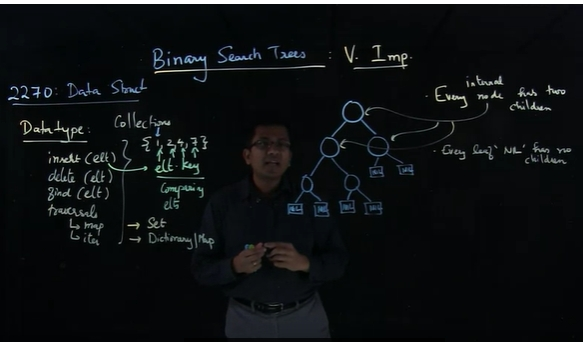
\includegraphics[width=\textwidth]{binarysearchtreenodes.png}
\end{figure}

\paragraph{
    When there is a node with the key 25, every node in the left subtree
    will have a key $<$ 25, and every node in the right subtree will
    have a key $>$ 25.\\
    The rule will also apply to all those subtrees.\\
}

\begin{figure}[H]
    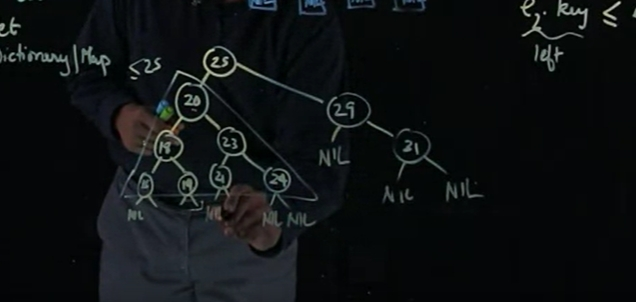
\includegraphics[width=\textwidth]{binarysearchtreerealexample.png}
\end{figure}

\begin{verbatim}
    Example:
     25
    /  \
   15  50
  / \  / \
 10 22 35 70
\end{verbatim}

\begin{verbatim}

Question:
Binary Search Trees may look similar to Heaps, but it is important 
to consider their differences.
In a Min-Heap, the smallest element must be the root node of the tree.
In a Binary Search Tree, on the other hand, how would we find the 
smallest element?

A: We would traverse the left subtree of the root node until we 
reach a leaf node, which means a node with a NIL as its left child.
\end{verbatim}


\subsection{The Height of a Binary Search Tree}

\paragraph{
    The height of a binary search tree is the number of edges on the
    longest path from the root node to a leaf node.\\
    We will define the height of a leaf node as 0. Then the height of number 25, 
    a.k.a. the root node of the below binary search tree is 2.\\
}

\newpage

\begin{verbatim}
    Example:
     25       -> height = 2
    /  \
   15  50     -> height = 1
  / \  / \
 10 22 35 70  -> height = 0, since they are leaf nodes
\end{verbatim}

\paragraph{
    Let's assume we have a balanced binary search tree with n internal nodes.\\
    One each layer from the root node, there'll be $2^0$ nodes, $2^1$ nodes, $2^2$ nodes, $\cdots$, $2^h$ nodes.\\
    The total number of nodes in the tree will be $2^0+2^1+2^2+ \cdots +2^h=2^{h+1}-1$.\\
    So, the height of the tree will be $h=\log_2(n+1)-1$.\\
    In the sense of big O notation, the height of a binary search tree is $O(\log_2(n))$, in a balanced binary 
    search tree scenario.\\
    For example, $\log_2^8=3$, so the height of a binary search tree with 8 nodes is 3.\\
    $\log_2^{15}=4$, so the height of a binary search tree with 15 nodes is 4.\\
}

\paragraph{
    In the worst case scenario, where the binary search tree is not balanced, the height of the tree will be $O(n)$.\\
    That is to say, the tree will be a linked list looks like this;\\
}

\newpage

\begin{verbatim}
    Linked List Example:
     10
      \
       15
        \
         20
          \
           25
            \
             30
              \
               35
\end{verbatim}

\paragraph{
    In this case, the height of the tree is 6, which is equal to the number of nodes in the tree.\\
    The height of the tree is $O(n)$, which is the worst case scenario.\\
    Normally, we will have something in between the best case scenario and the worst case scenario, 
    $O(\log(n)) < height < O(n)$.\\
}

\subsection{Basics of Binary Search Tree Quiz}

\begin{figure}[H]
    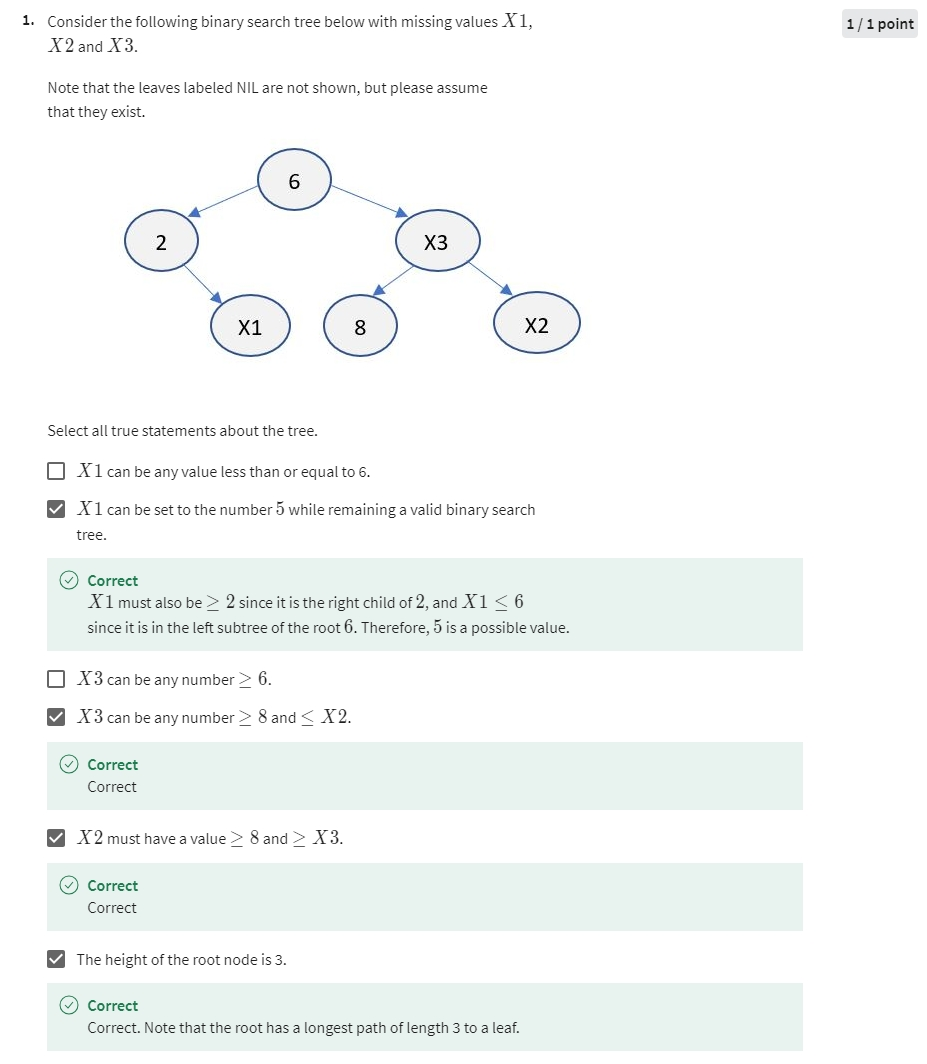
\includegraphics[width=\textwidth]{binarysearchtreequiz01.png}
\end{figure}

\begin{figure}[H]
    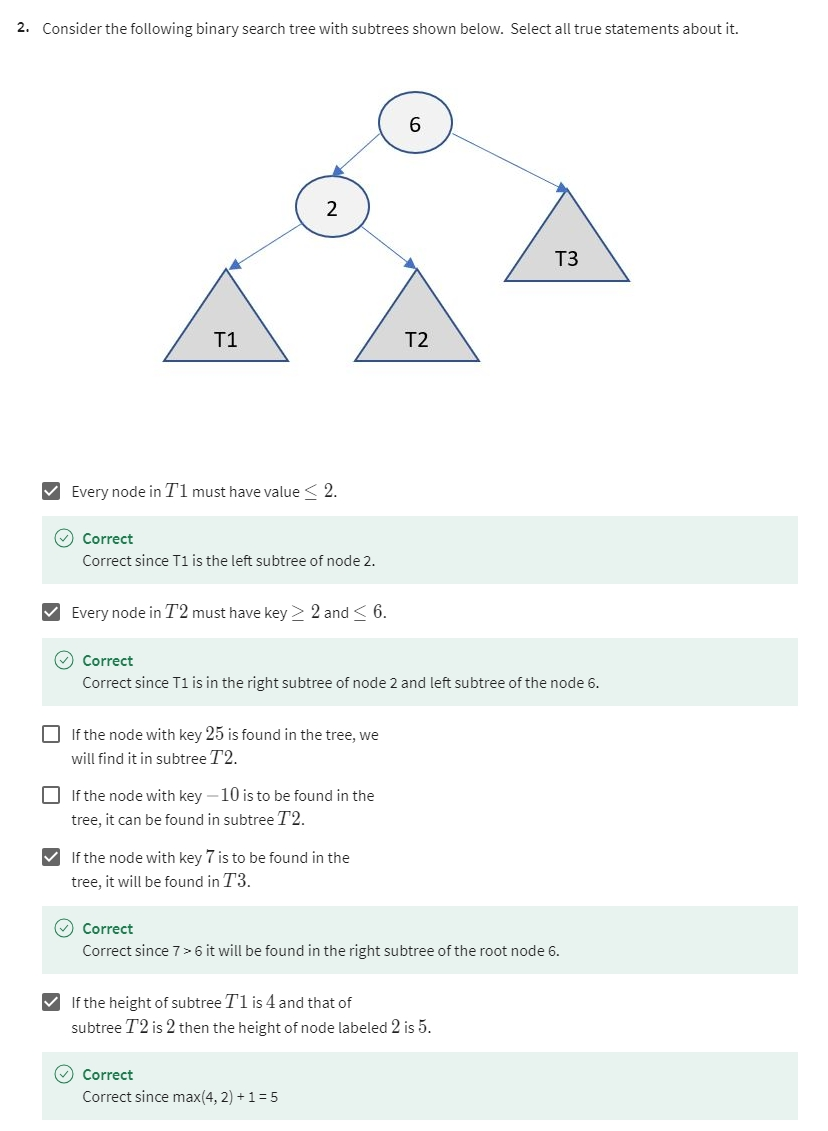
\includegraphics[width=\textwidth]{binarysearchtreequiz02.png}
\end{figure}

\begin{figure}[H]
    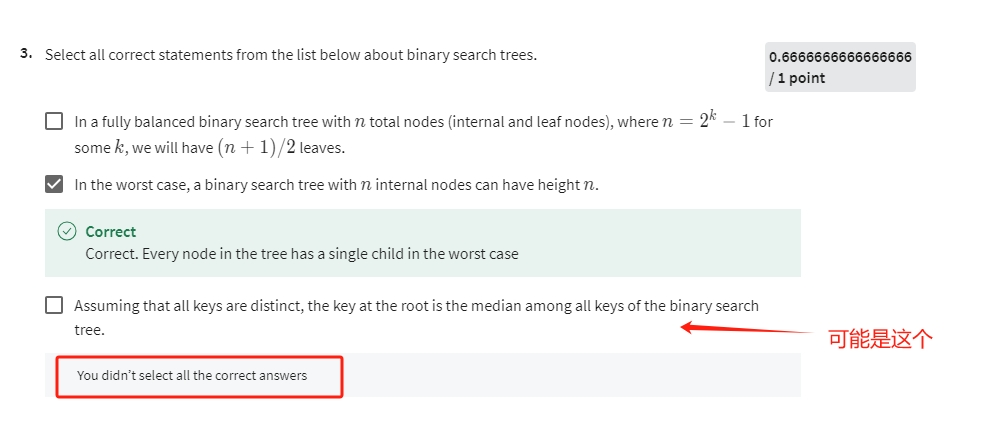
\includegraphics[width=\textwidth]{binarysearchtreequiz03.png}
\end{figure}



\subsection{Insertion and Deletion in a Binary Search Tree}

\subsubsection{Insertion}

\paragraph{
    We can insert a new element into a binary search tree by comparing the key of the new element with the key of the root node.\\
    If the key of the new element is less than the key of the root node, we will insert the new element into the left subtree.\\
    If the key of the new element is greater than the key of the root node, we will insert the new element into the right subtree.\\
    We will repeat the process until we reach a leaf node.\\
    For example, we have a binary search tree with the following nodes;\\
}

\begin{verbatim}
    Example:
     25
    /  \
   15  50
  / \  / \
 10 22 35 70
\end{verbatim}

\paragraph{
    If we want to insert a new element with the key 40, we will compare 40 with 25, and then 40 with 50, and then 40 with 35.\\
    Since 40 is greater than 35, we will insert 40 as the right child node of 35.\\
}

\paragraph{
    The above example actually consists of two steps.\\
    First, we will search for the element to be inserted, which is called the $find()$ operation.\\
    Then, after successfully locates the element, we will insert it into the binary search tree.\\
    We will talk about find operation now.\\
    Assuming we have an impefect binary search tree and we want to locate the key $45$, how should we do that?\\
}

\begin{figure}[H]
    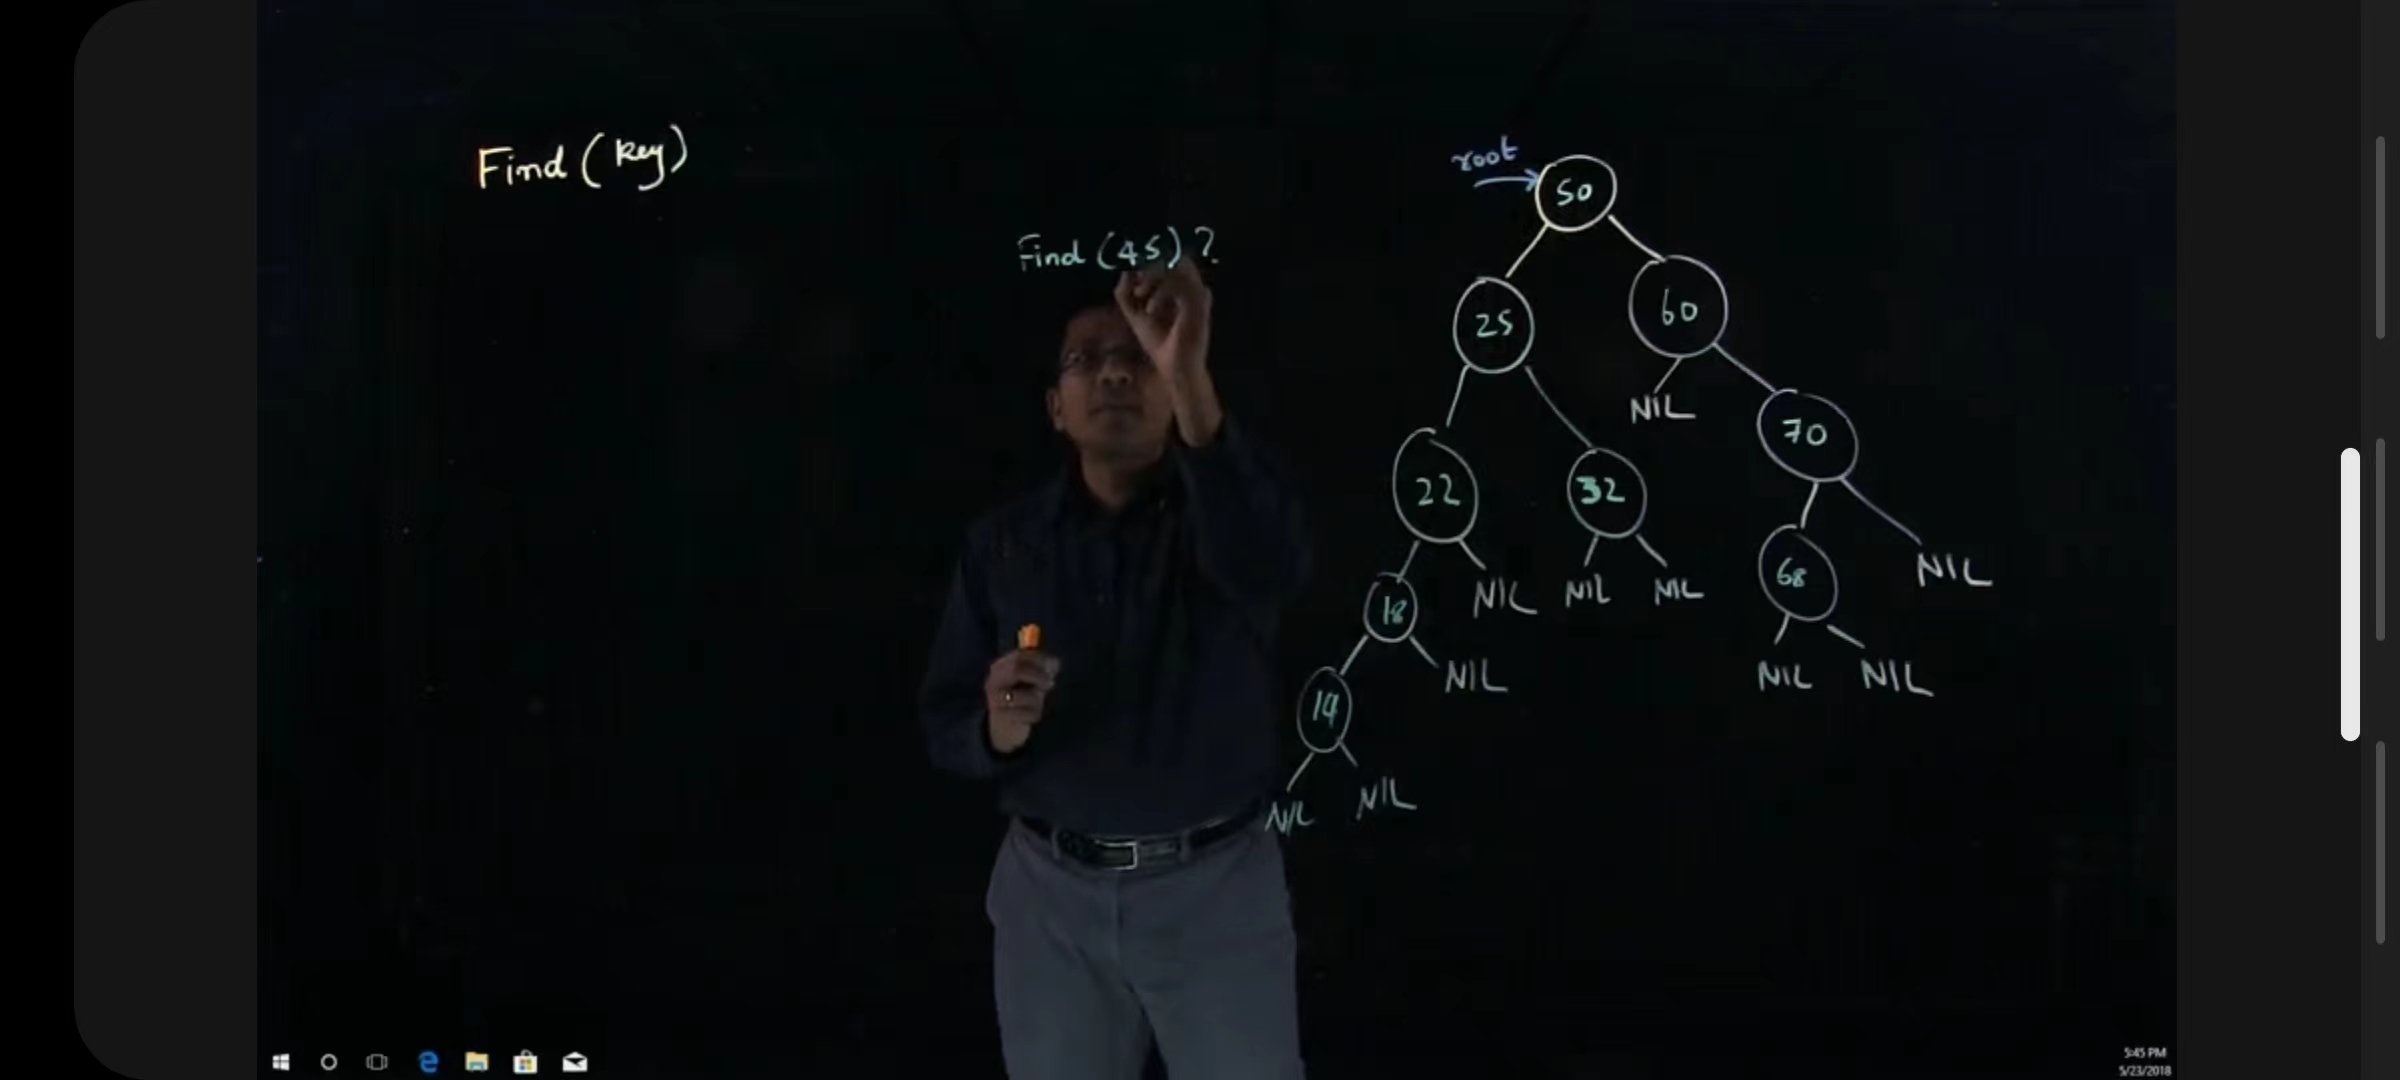
\includegraphics[width=\textwidth]{binarysearchtreeinsertion.jpg}
\end{figure}

\paragraph{
    We will start from the root node, and then compare the key of the root node with the key of the element to be located.\\
    If the key of the root node is equal to the key of the element to be located, we will return the root node. 
    If the key of the root node is greater than the key of the element to be located, we will search the left subtree. 
    Otherwise, we will search the right subtree.\\
    The overall process will be repeated until we reach a leaf node.\\
    If we reach a leaf node and the key of the leaf node is not equal to the key of the element to be located, we will return NIL.\\
}

\begin{verbatim}
    Here is the pseudo code for the find operation:
    find(root, key)
        if root == NIL or root.key == key
            return root
        if root.key > key
            return find(root.left, key) # This is the recursive call.
        return find(root.right, key) # This is the recursive call.
\end{verbatim}

\paragraph{
    As for the time complexity, the find operation will take $O(h)$ time, where $h$ is the height of the binary search tree.\\
    Now we will go ahead with the second step of the insertion operation.\\
    We will insert the new element into the binary search tree by comparing the key of the new element with the key of the root node.\\
    }

\begin{verbatim}
    Here is the pseudo code for the insertion operation:
    insert(root, key)
        if root == NIL
            return new Node(key)
        if key < root.key
            root.left = insert(root.left, key) # This is the recursive call.
        else
            root.right = insert(root.right, key) # This is the recursive call.
        return root
\end{verbatim}

\begin{figure}[H]
    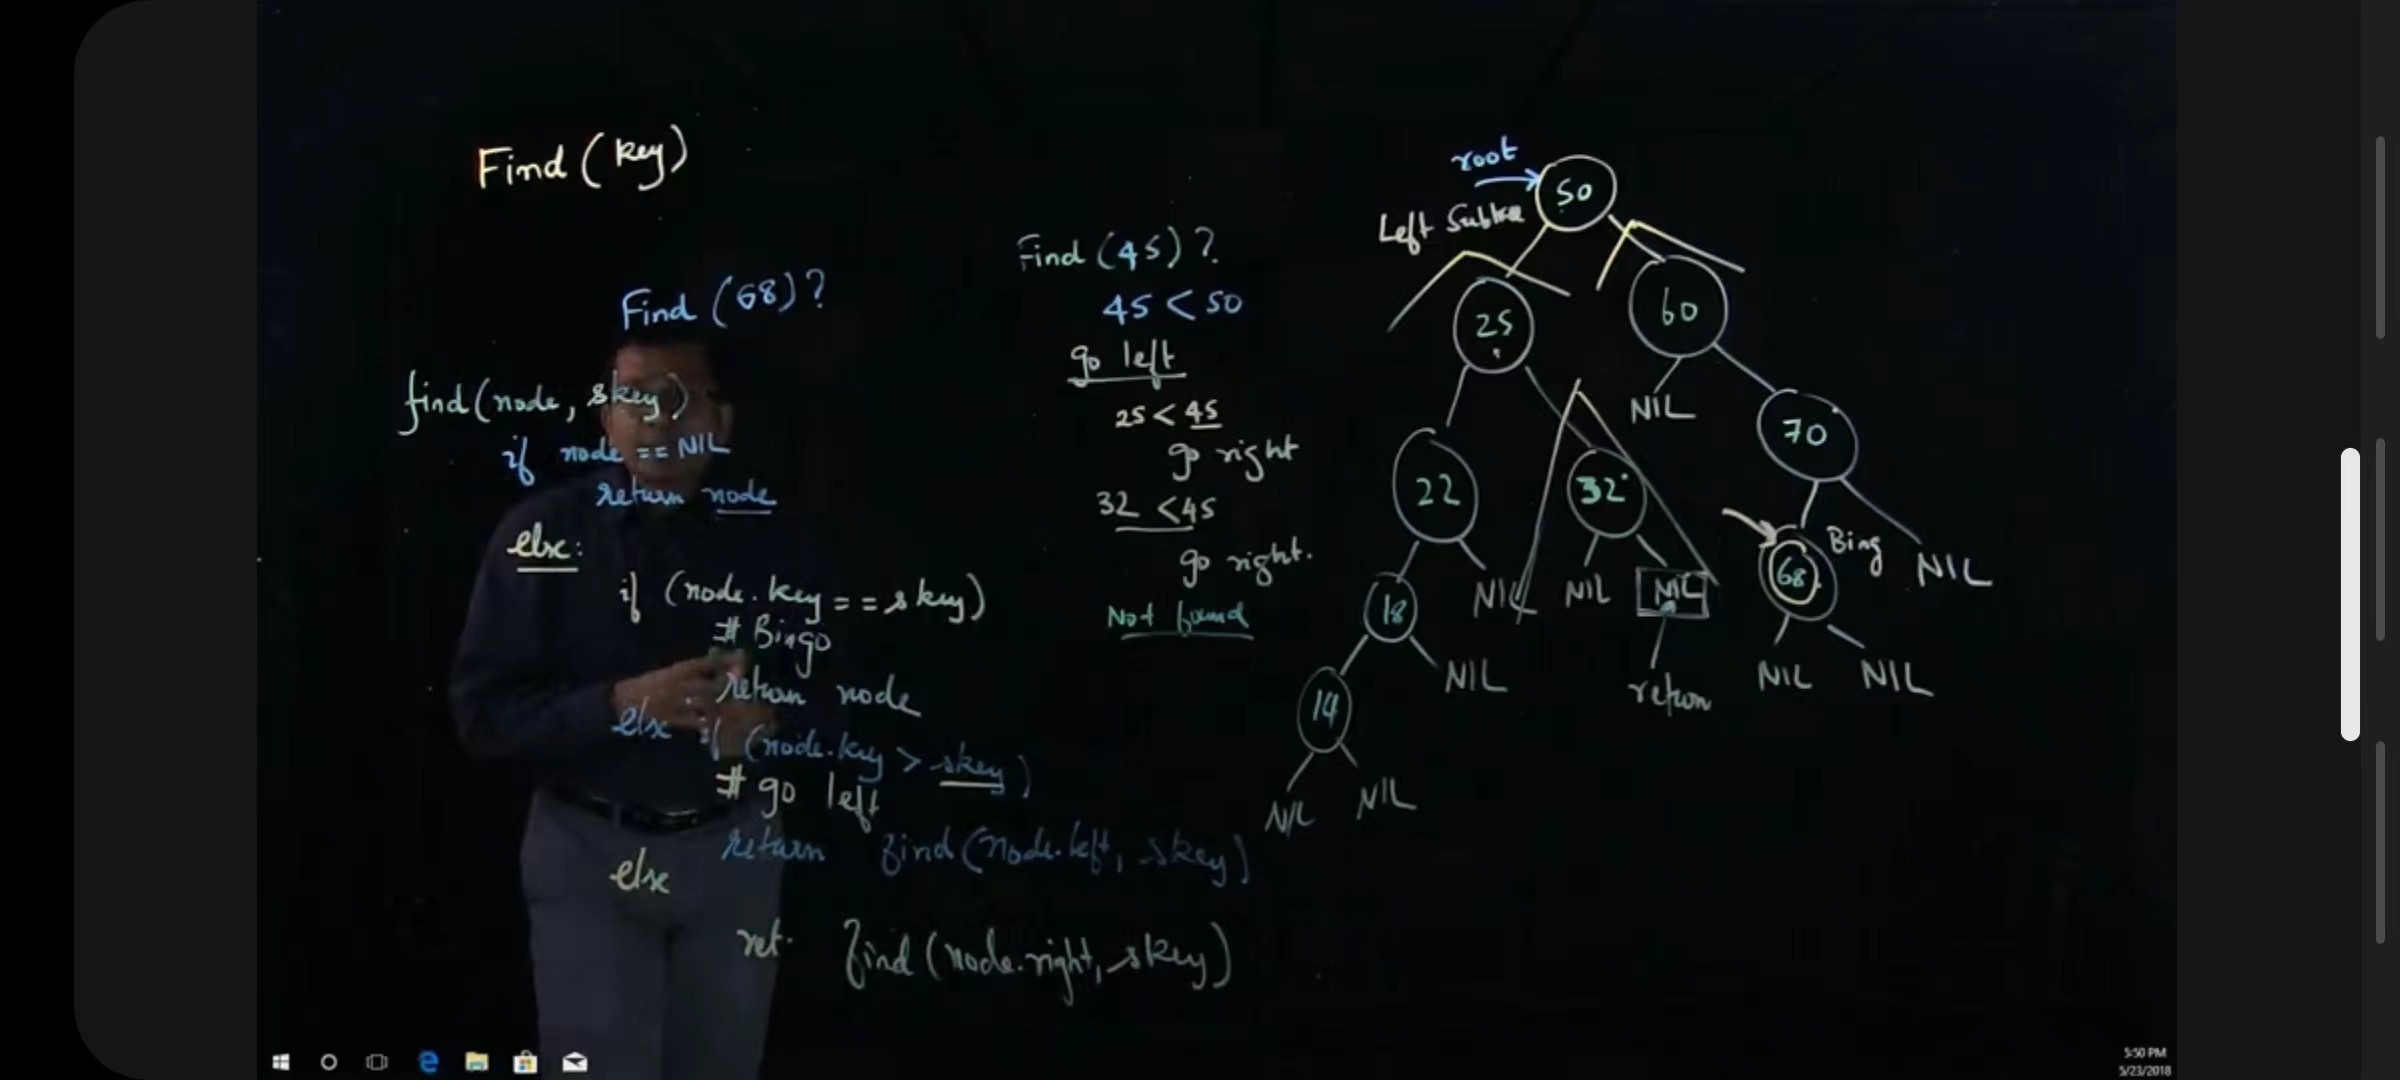
\includegraphics[width=\textwidth]{binarysearchtreeinsertion2.jpg}
\end{figure}

\subsubsection{Deletion}

\paragraph{
    Now we will talk about the deletion operation.\\
    There are three cases to consider when deleting a node from a binary search tree.\\
    The node to be deleted can be a leaf node, a node with only one child,or one with two child nodes.\\
    If both child nodes are NIL, we can simply delete the node.\\
    If one of the child nodes is NIL, we can delete the node, then reconnect between the past-parrent node and past-child node,
     like this;\\
}

\newpage

\begin{verbatim}
    Only One Child Node Example:
     25                     25
    /  \                   /  \
   15  50   delete 15     /   50
  / \       --------->   / \
 10 NIL                 10  NIL
 /\                    / \
NIL NIL               NIL NIL
\end{verbatim}

\paragraph{
    What if we want to delete a node that has two non-NIL children?\\
    We will find the smallest node in the right subtree of the node to be deleted, and then replace the node to be deleted with the smallest node.\\
    To perform this operation, we will `walk' right from the root node by one step and then `walk' left until we reach a leaf node.\\
    During each step, we will compare the key of the current node with the key of the node to be deleted.\\
    The leaf node we reached will be the successor of the node we deleted.\\
}

\begin{verbatim}
    Two Child Nodes Example:
     25                     25
    /  \                   /  \
   15  50   delete 15     22   50
  / \       --------->   / \
 10 22                 10  NIL
 /\                    / \
NIL NIL               NIL NIL
\end{verbatim}

\begin{verbatim}
    Here is the pseudo code for the deletion operation:
    delete(root, key)
        if root == NIL
            return root
        if key < root.key
            root.left = delete(root.left, key) # This is the recursive call.
        else if key > root.key
            root.right = delete(root.right, key) # This is the recursive call.
        else
            if root.left == NIL
                return root.right
            else if root.right == NIL
                return root.left
            root.key = minValue(root.right)
            root.right = delete(root.right, root.key) # This is the recursive call.
        return root
\end{verbatim}


\subsubsection{Tree Traversal}

\paragraph{
    There are three ways to traverse a binary search tree.\\
    In-order traversal, pre-order traversal, and post-order traversal.\\
    In-order traversal will visit the left subtree, then the root node, and then the right subtree.\\
    Pre-order traversal will visit the root node, then the left subtree, and then the right subtree.\\
    Post-order traversal will visit the left subtree, then the right subtree, and then the root node.\\
}



TBC: Binary search tree: insertion and deletion video: preorder traversal


\end{document}